\documentclass[12pt]{article}
\usepackage[dvipsnames]{xcolor}
\usepackage{tikz}
\usepackage{amsmath}
\usepackage{amsthm}
\usepackage{amssymb}
\usepackage{float}
\usepackage{titlesec}

\usepackage[strict]{changepage} 
\usepackage{framed} 

\usepackage{geometry}
\usepackage{url}
\usepackage{tcolorbox}
\setcounter{secnumdepth}{4}
\geometry{a4paper,scale=0.8}
\linespread{1}

\renewcommand{\baselinestretch}{1.4}

\definecolor{formalshade}{rgb}{0.95,0.95,1} % Shaded theorem background

\newenvironment{formal}{%
\def\FrameCommand{%
\hspace{1pt}%
{\color{Blue}\vrule width 2pt}%
{\color{formalshade}\vrule width 4pt}%
\colorbox{formalshade}%
}%
\MakeFramed{\advance\hsize-\width\FrameRestore}%
\noindent\hspace{-4.55pt}% 
\begin{adjustwidth}{}{7pt}%
\vspace{2pt}\vspace{2pt}%
}
{%
\vspace{2pt}\end{adjustwidth}\endMakeFramed%
}

\newcounter{mytheoremcounter}
\newcounter{mydefinitioncounter}
\newcounter{mylemmacounter}
%theorem
\newtcolorbox{mytheorem}[1][]{
    colback=blue!5!white,      
    colframe=Blue,    
    fonttitle=\bfseries,       
       title=Theorem~\refstepcounter{mytheoremcounter}\themytheoremcounter,  
    #1
}
%definition
\newtcolorbox{mydefinition}[1][]{
    colback=SpringGreen!5!white,     
    colframe=SpringGreen!88!black,     
    fonttitle=\bfseries,       
       title=Definition~\refstepcounter{mydefinitioncounter}\themydefinitioncounter,  
    #1
}

\newtcolorbox{mylemma}[1][]{
    colback=blue!5!white,     
    colframe=Blue,  
    fonttitle=\bfseries,       
       title=Lemma~\refstepcounter{mylemmacounter}\themylemmacounter,
    #1
}

\titleformat{\section}
  {\large\bfseries}
  {\thesection}    
  {1em}           
  {}               

\newtheorem{theorem}{Theorem}[section]
\newtheorem{definition}{Definition}[section]
\newtheorem{corollary}{Corollary}[theorem]
\newtheorem{lemma}[theorem]{Lemma}

\begin{document}
\begin{center}
\begin{large}
\textbf{Approximation by Superpositions of a Sigmoidal Function}\\
\end{large}
Notes by Zixin Yu
\end{center}

In 1989, Cybenko published \emph{Approximation by Superpositions of a Sigmoidal Function}~\cite{1}. He proved that a feedforward neural network with a single hidden layer and a continuous sigmoidal activation function can approximate any continuous function on the unit cube to arbitrary accuracy. This is a version of the \textbf{universal approximation theorem}. In these notes, I outline the proof, clarify points that I found confusing, and expand on details that Cybenko left implicit. The argument uses concepts from measure theory and functional analysis; I introduce the main results as they arise to make the proof easier to follow.

\section{Problem Description}

\begin{figure}[H]
    \centering
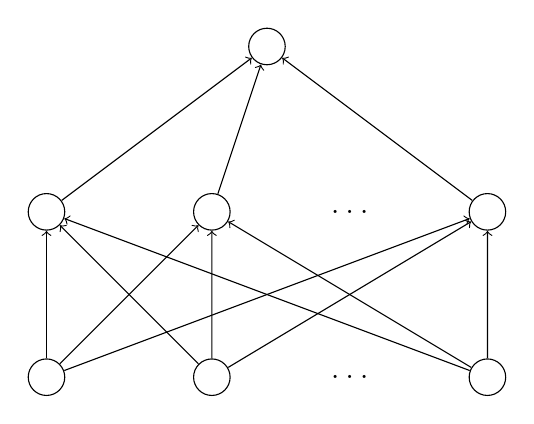
\begin{tikzpicture}[scale=1.4, every node/.style={scale=1.4}]

    \node[circle, draw] (input1) at (0, 0) {};
    \node[circle, draw] (input2) at (1.5, 0) {};
    \node[circle, draw] (input3) at (4, 0) {};
    
    \node[circle, draw] (hidden1) at (0, 1.5) {};
    \node[circle, draw] (hidden2) at (1.5, 1.5) {};
    \node[circle, draw] (hidden3) at (4, 1.5) {};
    \node[circle, draw] (output1) at (2, 3) {};
    
    \node at (2.75, 0) {\scriptsize \(\dots\)};
    \node at (2.75,1.50) {\scriptsize \(\dots\)};
    
    \draw[->] (input1) -- (hidden1);
    \draw[->] (input1) -- (hidden2);
    \draw[->] (input1) -- (hidden3);
    
    \draw[->] (input2) -- (hidden1);
    \draw[->] (input2) -- (hidden2);
    \draw[->] (input2) -- (hidden3);
    
    \draw[->] (input3) -- (hidden1);
    \draw[->] (input3) -- (hidden2);
    \draw[->] (input3) -- (hidden3);
    
    \draw[->] (hidden1) -- (output1);
    \draw[->] (hidden2) -- (output1);
    \draw[->] (hidden3) -- (output1);
    
    \end{tikzpicture}
\end{figure}

A feedforward neural network with a single hidden layer typically takes the following form:
\begin{align*}
    \sum_{j=1}^N \alpha_j \sigma (w_j^T x +\theta_j).
\end{align*}

Here, $x \in \mathbb{R}^n$ is the input, $w_j \in \mathbb{R}^n$ is the input weight vector for hidden neuron $j$, $\alpha_j \in \mathbb{R}$ is its output weight, and $\theta_j \in \mathbb{R}$ is its bias. The function $\sigma$ is the activation function, and $x \mapsto w_j^T x + \theta_j$ is an affine function of the input.

Let $I_n=[0,1]^n$ be the $n$-dimensional unit cube, and let $C(I_n)$ denote the space of real-valued continuous functions on $I_n$. Let $M(I_n)$ denote the space of finite signed regular Borel measures on $I_n$. For $f \in C(I_n)$, the supremum norm is $\lVert f\rVert_\infty=\max_{x\in I_n}|f(x)|$. Our goal is to determine when finite sums of the following form are dense in $C(I_n)$ with respect to the supremum norm:
\begin{align*}
    G(x)= \sum_{j=1}^N \alpha_j \sigma (w_j^T x +\theta_j).
\end{align*}

\begin{mydefinition}
A function $\sigma:\mathbb{R}\to\mathbb{R}$ is \emph{discriminatory} if, for every $\mu \in M(I_n)$, the condition
    \begin{align*}
        \int_{I_n} \sigma(w^Tx+\theta)\mathrm{d}\mu(x)=0
    \end{align*}
    for all $w \in \mathbb{R}^n$ and $\theta \in \mathbb{R}$ implies that $\mu = 0$.
\end{mydefinition}
I initially found this definition confusing. Equivalently, for every nonzero measure $\mu \in M(I_n)$, there exist $w \in \mathbb{R}^n$ and $\theta \in \mathbb{R}$ such that
\begin{align*}
\int_{I_n}\sigma(w^Tx+\theta)\mathrm{d}\mu(x)\neq 0.
\end{align*}
The quantifier ``for all $w$ and $\theta$'' is essential: a single vanishing integral does not imply that $\mu=0$. Intuitively, the family of functions $x\mapsto\sigma(w^Tx+\theta)$ can detect every nonzero finite signed regular Borel measure through integration. Now consider the definition of a sigmoidal function.

\begin{mydefinition}
    A sigmoidal activation function satisfies
    $$\sigma(t) \to 
    \begin{cases} 
    1, & t \to +\infty \\
    0, &  t \to -\infty.
    \end{cases}$$
\end{mydefinition}
The logistic function $\sigma(t)=1/(1+e^{-t})$ satisfies Definition 2. We will work with the general class of sigmoidal functions rather than a particular example. Section 2 presents the main results, and Section 3 applies them to neural networks. Cybenko also discusses other activation functions, which are beyond the scope of these notes.

\section{Main Results}

\begin{mytheorem}
    Let $\sigma$ be any continuous discriminatory function. Then finite sums of the form
    \begin{align}
        G(x)=\sum_{j=1}^N \alpha_j \sigma (w_j^T x +\theta_j)
    \end{align}
    are dense in $C(I_n)$. In other words, given any $f \in C(I_n)$ and $\varepsilon > 0$, there exists a function $G$ of the above form such that
    \begin{align*}
        |G(x)-f(x)|<\varepsilon, \quad x\in I_n.
    \end{align*}
\end{mytheorem}

\begin{proof}
    Let $S \subseteq C(I_n)$ be the set of all finite sums of the form (1). Then $S$ is a linear subspace of $C(I_n)$. To prove density, we must show that its closure $\overline{S}$ is all of $C(I_n)$. Suppose, for a contradiction, that $\overline{S} \neq C(I_n)$. Then $\overline{S}$ is a proper closed subspace of $C(I_n)$.
\begin{formal}
\textbf{A Consequence of the Hahn--Banach Theorem}\\
Let $X$ be a real normed vector space, and let $Y$ be a proper closed linear subspace of $X$. There exists a nonzero bounded linear functional $L:X\to\mathbb{R}$ such that $L(y)=0$ for every $y\in Y$.
\end{formal}

Applying this consequence of the Hahn--Banach theorem with $X=C(I_n)$ and $Y=\overline{S}$ gives a bounded linear functional $L$ on $C(I_n)$ such that
\begin{align*}
    L(h)=0\quad\text{for every }h\in\overline{S},\qquad L\neq 0.
\end{align*}

\begin{formal}
\textbf{Riesz Representation Theorem}\\
Let $K$ be a compact Hausdorff space. Every bounded linear functional $L$ on the real-valued continuous functions $C(K)$ has a unique representation
\[
L(h)=\int_K h(x)\,\mathrm{d}\mu(x),\qquad h\in C(K),
\]
where $\mu$ is a finite signed regular Borel measure on $K$.
\end{formal}
The Riesz representation theorem gives a measure $\mu\in M(I_n)$ with
\begin{align*}
    L(h)=\int_{I_n} h(x)\mathrm{d}\mu(x),\qquad h\in C(I_n).
\end{align*}
For every $w\in\mathbb{R}^n$ and $\theta\in\mathbb{R}$, the function $x\mapsto\sigma(w^T x + \theta)$ belongs to $S$. Since $L$ vanishes on $S$,
\begin{align*}
    \int_{I_n} \sigma(w^Tx+\theta)\mathrm{d}\mu(x)=0.
\end{align*}
Since $\sigma$ is discriminatory, $\mu = 0$. This contradicts $L \neq 0$, because
\begin{align*}
    \mu=0 \implies L(h)=\int_{I_n} h(x)\mathrm{d}\mu(x)=0,\quad h\in C(I_n).
\end{align*}
Therefore, $S$ is dense in $C(I_n)$. 
\end{proof}

\begin{mylemma}
    Any continuous sigmoidal function is discriminatory.
\end{mylemma}
To prove this lemma, we assume that a measure annihilates every function $x\mapsto\sigma(w^Tx+\theta)$ and show that the measure is zero. The key is to rescale the inputs to $\sigma$ and use dominated convergence to obtain information about the measures of half-spaces.

\begin{proof}
    Suppose $\mu\in M(I_n)$ satisfies
\[
\int_{I_n}\sigma(w^Tx+\theta)\,\mathrm{d}\mu(x)=0
\quad\text{for every }w\in\mathbb{R}^n,\ \theta\in\mathbb{R}.
\]
Fix $w\in\mathbb{R}^n$ and $\theta,\varphi\in\mathbb{R}$. By the sigmoidal limits,
\begin{align*}
    \sigma(\lambda (w^T x + \theta) + \varphi) \rightarrow 
\begin{cases}
1, &  \quad w^T x + \theta > 0 \quad \text{as} \quad \lambda \to +\infty, \\
0, &  \quad w^T x + \theta < 0 \quad \text{as} \quad \lambda \to +\infty, \\
\sigma(\varphi), & \quad w^T x + \theta = 0 \quad \text{for all} \quad \lambda.
\end{cases}
\end{align*}
Thus, as $\lambda \to +\infty$, the functions $\sigma_\lambda(x)=\sigma(\lambda (w^T x + \theta) + \varphi)$ converge pointwise to
\begin{align*}
    \gamma(x) =
\begin{cases}
1, & \quad w^T x + \theta > 0, \\
0, & \quad w^T x + \theta < 0, \\
\sigma(\varphi), & \quad w^T x + \theta = 0.
\end{cases}
\end{align*}
Define the level set $\Pi_{w,\theta} = \{x \in I_n : w^T x + \theta = 0\}$ and the set $H_{w,\theta} = \{x \in I_n : w^T x + \theta > 0\}$. When $w\neq0$, these are the intersections of $I_n$ with a hyperplane and an open half-space, respectively.

Because $\sigma$ is continuous and has finite limits at $\pm\infty$, it is bounded on $\mathbb{R}$. Let $M=\sup_{t\in\mathbb{R}}|\sigma(t)|<\infty$. Then $|\sigma_\lambda(x)|\leq M$, and this constant is integrable with respect to the finite total variation measure $|\mu|$. Moreover, the hypothesis gives $\int_{I_n}\sigma_\lambda\,\mathrm{d}\mu=0$ for every $\lambda>0$, since the rescaled weight and bias are $\lambda w$ and $\lambda\theta+\varphi$. Dominated convergence therefore gives
\begin{align*}
    0&=\lim_{\lambda\to \infty} \int_{I_n} \sigma_\lambda(x)\mathrm{d}\mu(x)\\
    &= \int_{I_n} \lim_{\lambda\to \infty} \sigma_\lambda(x)\mathrm{d}\mu(x)\\
    &=\int_{I_n} \gamma(x) \mathrm{d}\mu(x)\\
    &=\sigma(\varphi)\mu(\Pi_{w,\theta})+\mu(H_{w,\theta}).
\end{align*}
This identity holds for every $\varphi$. Letting $\varphi\to-\infty$ yields $\mu(H_{w,\theta})=0$, and then letting $\varphi\to+\infty$ yields $\mu(\Pi_{w,\theta})=0$. We now show that these identities force $\mu$ to be the zero measure.

Fix $w$. For a bounded Borel measurable function $h:\mathbb{R}\to\mathbb{R}$, define the linear functional
\begin{align*}
    F(h) = \int_{I_n} h(w^T x) \, \mathrm{d}\mu(x).
\end{align*}
Since
\begin{align*}
\left|F(h)\right| &= \left|\int_{I_n} h(w^T x) \, \mathrm{d}\mu(x)\right| \\
&\leq \int_{I_n}|h(w^Tx)|\,\mathrm{d}|\mu|(x) \\
&\leq \lVert h\rVert_\infty\,|\mu|(I_n),
\end{align*}
the functional $F$ is bounded in the supremum norm. Here $\lVert h\rVert_\infty=\sup_{t\in\mathbb{R}}|h(t)|$, and $|\mu|(I_n)$ is finite because $\mu$ is a finite signed measure.

Let $h$ be the indicator function of $[\theta,+\infty)$, that is,
\begin{align*}
    h(t) = \begin{cases}
        1, & t \geq \theta, \\
        0, & t < \theta.
    \end{cases}
\end{align*}
Using the identities for the measures of the level sets and half-spaces, we obtain
\begin{align*}
    F(h) &= \int_{I_n} h(w^T x) \, \mathrm{d}\mu(x) \\
    &= \mu(\Pi_{w, -\theta}) + \mu(H_{w, -\theta}) \\
    &= 0.
\end{align*}
Similarly, if $h$ is the indicator function of $(\theta,+\infty)$, then $F(h)=\mu(H_{w,-\theta})=0$. Write $h_E$ for the indicator function of an interval $E$. For $a<b$,
\begin{align*}
    h_{[a,b]}&=h_{[a,+\infty)}-h_{(b,+\infty)},\\
    h_{(a,b)}&=h_{(a,+\infty)}-h_{[b,+\infty)}.
\end{align*}

By linearity, $F(h_{[a,b]})=F(h_{(a,b)})=0$. The same argument applies to half-open intervals and singletons. Thus, for any finite interval step function $r=\sum_{j=1}^N a_j h_{E_j}$,
$$
F(r)=\sum_{j=1}^N a_jF(h_{E_j})=0.
$$
The set $J_w=\{w^Tx:x\in I_n\}$ is a compact interval, possibly a single point. Every continuous function $h$ on $J_w$ can be approximated uniformly there by interval step functions $r_k$. Extending $h$ and $r_k$ by zero outside $J_w$ allows us to apply $F$, and the bound
\begin{align*}
    |F(h)-F(r_k)|\leq |\mu|(I_n)\sup_{t\in J_w}|h(t)-r_k(t)|\longrightarrow0
\end{align*}
shows that $F(h)=0$. In particular, this applies to the restrictions of sine and cosine to $J_w$. Since $w$ was arbitrary, the Fourier transform of $\mu$, extended by zero outside $I_n$, satisfies
\begin{align*}
    \hat{\mu}(w)&=\int_{I_n} e^{-iw^Tx}\mathrm{d}\mu(x)\\
    &=\int_{I_n} \cos(w^Tx)\mathrm{d}\mu(x)-i\int_{I_n} \sin(w^Tx)\mathrm{d}\mu(x)\\
    &=F(\cos)-iF(\sin)\\
    &=0,\qquad w\in\mathbb{R}^n.
\end{align*}
By uniqueness of the Fourier transform for finite measures, $\mu=0$. Therefore, every continuous sigmoidal function is discriminatory.
\end{proof}

\section{Application to Artificial Neural Networks}

\begin{mytheorem}
    Let $\sigma$ be any continuous sigmoidal function. Then finite sums of the form
\begin{align*}
G(x) = \sum_{j=1}^{N} \alpha_j \sigma(w_j^T x + \theta_j)
\end{align*}
are dense in $C(I_n)$. In other words, given any $f \in C(I_n)$ and $\varepsilon > 0$, there exists a function $G$ of the above form such that
\begin{align*}
|G(x) - f(x)| < \varepsilon, \quad x \in I_n.
\end{align*}
\end{mytheorem}

\begin{proof}
    By Lemma 1, every continuous sigmoidal function is discriminatory, so Theorem 1 applies.
\end{proof}

We have proved that a feedforward neural network with a single hidden layer and a continuous sigmoidal activation function can approximate any continuous function on $I_n$ uniformly. We now turn to classification, a fundamental task in machine learning. Let $m$ denote Lebesgue measure on $I_n$, and let $P_1,\dots,P_k$ be a measurable partition of $I_n$: the sets are pairwise disjoint and their union is $I_n$. Define the decision function $f$ by
\begin{align*}
    f(x) = j \quad \text{if and only if} \quad x \in P_j.
\end{align*}
The value $f(x)$ assigns a class label to $x$. This function need not be continuous, so Theorem 2 does not apply directly. Theorem 3 shows that a network can approximate $f$ outside a set of arbitrarily small measure.
\begin{mytheorem}
    Let $\sigma$ be a continuous sigmoidal function, and let $f$ be the decision function associated with a finite measurable partition of $I_n$. For any $\varepsilon > 0$, there exists a function of the form
\begin{align*}
G(x) = \sum_{j=1}^{N} \alpha_j \sigma(w_j^T x + \theta_j)
\end{align*}
and a measurable set $D \subseteq I_n$ such that $m(D) \geq 1 - \varepsilon$ and
\begin{align*}
|G(x) - f(x)| < \varepsilon,\qquad x\in D.
\end{align*}
\end{mytheorem}

\begin{proof}
    We use the following form of Lusin's theorem.
    \begin{formal}
        \textbf{Lusin's Theorem}\\
        Let $E\subseteq\mathbb{R}^n$ be a measurable set of finite Lebesgue measure, and let $g:E\to\mathbb{R}$ be measurable. For every $\delta>0$, there exists a compact set $D\subseteq E$ such that $m(E\setminus D)<\delta$ and the restriction $g|_D$ is continuous.
    \end{formal}
    Applying Lusin's theorem with $E=I_n$ and $\delta=\varepsilon$ gives a compact set $D\subseteq I_n$ with $m(D)\geq1-\varepsilon$ on which $f$ is continuous. By the Tietze extension theorem, the continuous function $f|_D$ extends to a function $h\in C(I_n)$. By Theorem 2, there is a network function $G$ such that $|G(x)-h(x)|<\varepsilon$ for every $x\in I_n$. Hence, for $x\in D$,
    $$
    |G(x) - f(x)| = |G(x) - h(x)| < \varepsilon.
    $$
    \end{proof}

\section{Conclusion}
Hornik's 1991 paper~\cite{hornik1991} extended uniform approximation results to continuous, bounded, nonconstant activation functions, showing that the sigmoidal limits are not essential. A single hidden layer still suffices, provided that sufficiently many hidden units are available. Universal approximation is an existence result: under the stated assumptions, a network can approximate a target function to arbitrary accuracy. It does not, by itself, specify how many neurons are needed or how to train the network to find suitable weights. Understanding this ``universality'' therefore requires attention to both approximation theory and practical learning methods.

\begin{thebibliography}{99}
    \bibitem{1} Cybenko, G. (1989). Approximation by superpositions of a sigmoidal function. \emph{Mathematics of Control, Signals, and Systems}, 2(4), 303--314. \url{https://doi.org/10.1007/BF02551274}
    \bibitem{hornik1991} Hornik, K. (1991). Approximation capabilities of multilayer feedforward networks. \emph{Neural Networks}, 4(2), 251--257. \url{https://doi.org/10.1016/0893-6080(91)90009-T}
\end{thebibliography}

\end{document}
